\hfill \break

{\LARGE Demo Description}\\

In order to obtain sufficient amount of training and test data, while guaranteeing experimental repeatability and efficiency, we created a suite of software tools to automate emulation experiments in a Cloud testbed, which can automatically create a large-scale OSPF-enabled virtual network system, initiate data transfers between end hosts, and inject arbitrary integrity errors into the virtual router interfaces and end hosts.  

Our main design objectives is to automate the experiment creation, configuration, and data collection at any given scale. This not only guarantees repeatable experiments at different scales, but also makes data manipulation for ML model training for RCA much more efficient.   

We will demonstrate the three main components of the emulation and RCA analysis system. An emulation experiment in ExoGENI testbed is depicted in Fig.~\ref{fig:chaosjungle}.

\subsection{Network creation and configuration}
An arbitrary topology can be created with nodes in the form of virtual machines (VM) running customized images. We leverage the Postboot scripting capability offered by ExoGENI testbed to automate the network configuration.  

In our experimental topology, we use a set of end hosts to emulate the OSG data sources and sinks, a virtual network consisting of core routers emulating the backbone network service providers (Internet2, ESNet, etc) and access routers emulating the access network service providers (regional research and education networks and campus networks). All nodes are connected with virtual layer-2 links with certain throughput guarantee as the private data plane. An extra management plane interface is also available on every node, which provides remote access from the public Internet. The end hosts run an Ubuntu image with our Chaos Jungle fault injection tools. The routers run an Ubuntu image with the Zebra software router and our Chaos Jungle fault injection tools.

At the virtual node booting time, our customized Postboot scripts automate the following steps: (1) detect all the interfaces and their IP addresses, and all the neighboring nodes and the links; (2) create the configuration files for Zebra and OSPF daemons and start the routing control plane at the router nodes; (3) detect and add the default routes at the end host nodes.    

ExoGENI provides an API to launch any given experimental topology. On a successful execution, our experimental topology will be up and running with routing configured and network reachability established among all end hosts.   

\subsection{Data transfer and fault injection}
For every experiment, we attach a controller node that can reach all the nodes in the topology via the management plane interface. The controller is provided a Postboot script that automatically learns the experimental topology, creates a list of end hosts, routers, and links, and populates the end hosts with a set of files for the data transfer.

A user can log into the controller node, modify the experimental configuration files that define the data origin and sink nodes, the list of nodes to introduce storage integrity error, the list of network link interfaces to be disrupted by the Chaos Jungle tool, and the fault injection probability.

Then the experiment software can be started to inject the fault, transfer the data files from the origins, check the integrity at the sinks, and collect the data. This sequence is repeated for every fault specified in the configuration file.

\begin{figure}[!ht]
\begin{center}
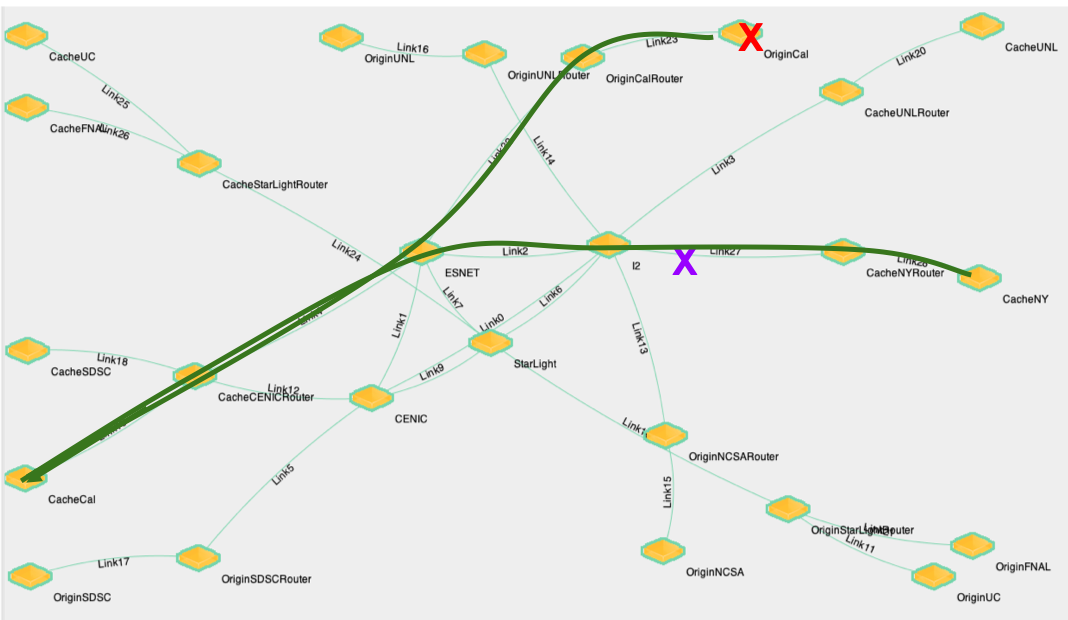
\includegraphics[width=0.48\textwidth]{./figure/ChaosJungle}
\end{center}
\caption{Network Emulation and Integrity Error Injection in ExoGENI}
\label{fig:chaosjungle}
\end{figure}

\subsection{Data collection and analysis}
At the last step, all the raw data will be processed and stored in final result database files with predefined feature columns. Each database entry represents one data transfer with features of file name, file size, origin, sink, access router, integrity error or not, etc. However, the forwarding path is unknown as it is controlled by the routing control plane process. The final result is exported to a Jupyter notebook environment where machine learning based data analysis is performed.

\hfill \break

{\LARGE Demo Set-Up}\\

The default display set-up plus Internet access is sufficient for our demonstration needs as we only run the client at the demo site. The actual experiments will be run in the remote Cloud.

